%!TEX root = ../index.tex

Die IT Abteilung in der allink wurde 2010 komplett neu gebildet. Zu diesem Zeitpunkt wurden ebenfalls grundlegende Technologie-Entscheide neu gefällt. Seitdem wurde die Produktivität der Webentwicklern stetig gesteigert und die Qualität verbessert. Dies indem Programmteile, welche in jedem Projekt wieder benötigt werden, nicht mehr für jedes Projekt neu erstellt werden und das Aufsetzen von neuen Projekten automatisiert wurde. Zudem existieren Werkzeuge welche wiederkehrende Tasks wie das Bereitstellen einer Webseite auf einem produktiv Server, oder das Einrichten einer lokalen Entwicklungsumgebung automatisieren.

\section{Eingesetzte Technologie Backend}
\label{sec:eingesetzte_technologie_backend}
Der grösste Teil aller Webprojekte in der allink werden mit Hilfe des Django Frameworks realisiert. Durch diese Wahl ergibt sich Python als präferierte Programmiersprache für alle serverseitigen Applikationen. Zudem wird FEINcms in allen Projekten eingesetzt welche eine cms Lösung benötigen. Hinergrundprozesse werden seit 2011 mit celery umgesetzt was gegenüber durch cronjobs ausgelöste Scripte einige Vorteile mit sich bringt. Weitere Applikationen, welche backendseitig in der allink häufig eingesetzt werden, sind in der Tabelle~\ref{tab:backend_applications} aufgeführt.

\begin{table}[ht]
  \centering
  \begin{tabular}{ll}
  \toprule
    Name & Link\\
  \midrule
    FEINcms & \url{http://www.feincms.org/}\\
  \midrule
    Pennyblack & \url{https://github.com/allink/pennyblack}\\
  \midrule
    Django Admin SSO & \url{https://github.com/frog32/django-admin-sso}\\
  \midrule
    South & \url{http://south.aeracode.org/}\\
  \midrule
    Django Robots & \url{https://github.com/jezdez/django-robots}\\
  \midrule
    Django Compressor & \url{https://github.com/jezdez/django_compressor/}\\
  \midrule
    cssmin & \url{https://github.com/zacharyvoase/cssmin}\\
  \midrule
    raven & \url{https://github.com/getsentry/raven-python}\\
  \midrule
    Celery & \url{http://www.celeryproject.org/}\\
  \bottomrule
  \end{tabular}
  \caption{Im backend häufig verwendete Applikationen}
  \label{tab:backend_applications}
\end{table}

\section{Eingesetzte Technologie Frontend}
\label{sec:eingesetzte_technologie_frontend}
Im frontend Bereich sind die eingesetzten Mittel mannigfaltiger als im backend Bereich. Hier kommt unter anderem das  Java Script Frameworks backbone.js~\footnote{\url{http://backbonejs.org/}} zum Einsatz. Für viele Projekte wird jedoch auch nur JQuery~\footnote{\url{http://jquery.com/}} verwendet. Weiterhin werden Tools wie Twitter Bootstrap~\footnote{\url{http://getbootstrap.com/}} sowie die Stylesheet Sprache less~\footnote{\url{http://lesscss.org/}} eingesetzt.

\section{Produktiv Systeme}
\label{sec:produktiv_systeme}
Die allink setzt für alle produktiven Web Systeme auf Managed Hosting von Nine Internet Solutions AG \footnote{http://nine.ch}. Von Nine wird die Verfügbarkeit der Serversysteme sichergestellt und Unterhaltsarbeit geleistet. Auch Backups der produktiven Systeme werden von Nine erstellt und archiviert.

\begin{table}[ht]
  \centering
  \begin{tabular}{ll}
  \toprule
    Softwarepaket & Version\\
  \midrule
    Apache & 2.2\\
  \hline
    Python & 2.7\\
  \hline
    libapache2-mod-wsgi & 3.3\\
  \hline
    MySQL Server & 5.5\\
  \hline
    Redis & 2.2\\
  \hline
    RabbitMQ & 2.7\\
  \bottomrule
  \end{tabular}
  \caption{Eingesetzte Softwareversionen}
  \label{tab:eingesetzte_softwareversionen}
\end{table}

\section{Eingesetzte Mittel für die Qualitätssicherung}
\label{sec:eingesetzte_mittel_für_die_qualitätssicherung}
Qualitätssicherung war in der allink schon immer ein Thema. Ab dem Zeitpunkt seit dem die allink Django einsetzt, wurden einige Bemühungen getätigt, um die Qualität zu gewährleisten. Die Tabelle~\ref{tab:qm_eingesetzte_mittel} zeigt eine Übersicht der Mittel, welche standardmässig bei jedem Webprojekt zum Einsatz kommen. Diese sind meist in das allink-project, ein Django Projekt welches die Grundlage für alle in der allink entwickelten Webapplikationen ist, integriert.

\makeatletter
\newcounter{bcounter}
\newcounter{bnumber} \setcounter{bnumber}{0}
\renewcommand\thebnumber{B\arabic{bnumber}}
\newcommand{\newbnumber}[3]%
{%
\midrule%
\refstepcounter{bnumber}\label{b:#2}%
\expandafter\xdef\csname b#2\endcsname {#1}%
\thebnumber & #1 & #3 \\
}
\makeatother


\begin{longtable}{l>{\raggedright}p{3cm}p{10cm}}
    \toprule \textbf{Nr.} & \textbf{System} & \textbf{Beschreibung} \\
    \newbnumber{unittests}{Unittests}{Business Logik wird wo vorhanden mittels Unittests getestet}
    \newbnumber{Precommit Hook}{precommithook}{Quellcode wird vor dem einchecken statisch ausgewertet und auf Konformität mit dem Syleguide geprüft.}
    \newbnumber{Sentry}{sentry}{Fehlermeldungen sämtlicher Webprojekte werden zentral mit Sentry aggregiert.}
    \newbnumber{Go-Live - Checkliste}{golivecheckliste}{Für den Go-Live einer Webseite besteht ein ausführliches Testprotokoll.}
    \newbnumber{Deployment Prozess}{deploymentprozess}{Der Deployment-Prozess wurde so implementiert, dass er einige Probleme selber erkennen kann.}
    \bottomrule
    \caption[Eingesetze Mittel]{Eingesetzte Mittel}
    \label{tab:qm_eingesetzte_mittel}
\end{longtable}

\subsection{Precommit Hook}
\label{sub:precommit_hook}
Der Precommit Hook überprüft den Quellcode eines Projektes vor jedem Commit. Dabei werden die Tools pyflake, pep8 und jshint eingesetzt um Python und Javascript Code zu verifizieren und zu überprüfen ob der Styleguide eingehalten wurde. Zudem wird im Quellcode nach debugging Anweisungen gesucht da diese nicht in einem Produktiv System laufen sollten.

\subsection{Sentry}
\label{sub:sentry}
Sentry ist ein zentrales Tool welches die Fehlermeldungen von sämtlichen Webprojekten der allink in einer Liste zusammenfasst. Sich wiederholende Fehler werden zusammengefasst, sodass man eine Übersicht erhält welcher Fehler wie häufig aufgetaucht ist. Die zentrale Fehlerliste von Sentry ist auf Abbildung~\ref{fig:sentry_index} zu sehen.

\begin{figure}[h]
\centering
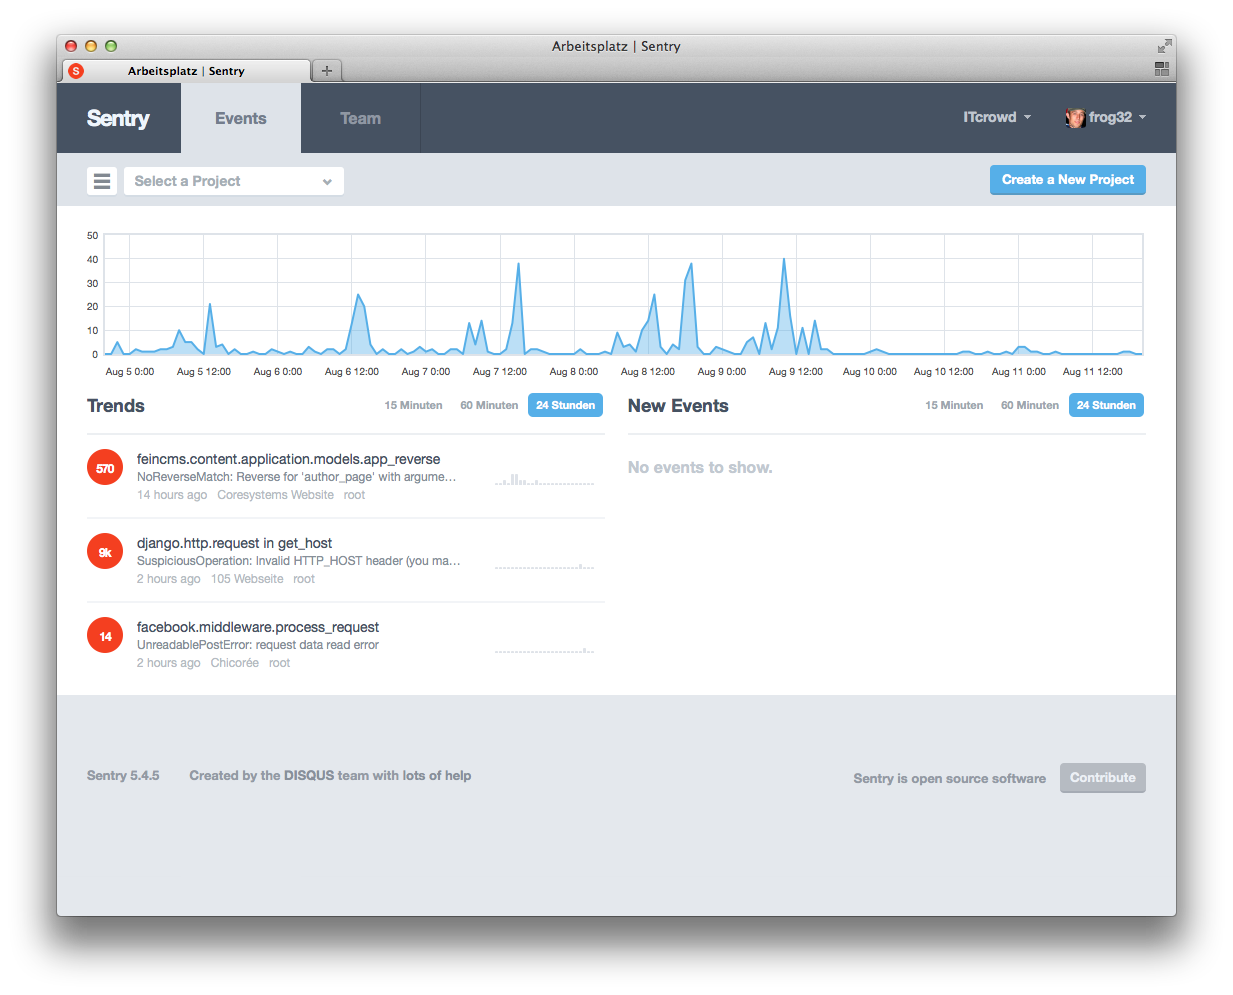
\includegraphics[width=1\textwidth]{images/sentry.png}
\caption{Sentry Übersicht}
\label{fig:sentry_index}
\end{figure}

\subsection{Go-Live - Checkliste}
\label{sub:go_live_checkliste}
Eine der ersten Massnahmen zur Qualitätssteigerung war das Einführen einer Checkliste, welche vor dem GoLive einer Webseite durchgearbeitet wird. Diese Überprüfung wird falls möglich von einem Entwickler welcher nicht am Projekt beteiligt war durchgeführt. Diese Checkliste wird laufend erweitert und ist zum Zeitpunkt dieser Arbeit 38 Punkte lang und in Anhang~\ref{sec:appendix_go_live_checkliste} zu sehen.

\subsection{Deployment Prozess}
\label{sub:deployment_prozess}
Mit dem Tool fabric wurde das Deployment in der allink weitmöglichst automatisiert. Lediglich das Einrichten der benötigten DNS Einträge und das Erstellen der Datenbank ist noch Handarbeit und wird jeweils beim erstmaligen Bereitstellen einer Webseite erledigt. Da bei diesem automatisierten Deployment unter anderem auch css Dateien minimiert werden, wird man beim Ausliefern einer Webseite auf css Fehler aufmerksam gemacht.